\documentclass{article}

\usepackage{amssymb}
\usepackage{amsmath}
\usepackage{graphicx}
\usepackage{mathptmx}
\usepackage{lipsum}  % for sample text
\usepackage[T1]{fontenc}
\usepackage{textcomp}
\usepackage{dirtytalk}

%include these lines if you want to use the LaTeX "theorem" environments
\newtheorem{theorem}{Theorem}[section]
\newtheorem{definition}[theorem]{Definition}
\newtheorem{lemma}[theorem]{Lemma}
\newtheorem{corollary}[theorem]{Corollary}


%include lines like this if you want to define your own commands 
%to save typing
\newcommand{\PROOF}{\noindent {\bf Proof}: }
\newcommand{\REF}[1]{[\ref{#1}]}
\newcommand{\Ref}[1]{(\ref{#1})}
\newcommand{\dt}{\mbox{\rm   dt}}
\newcommand{\phat}{\hat{p}}


 \usepackage{setspace}
 \onehalfspacing
 \newtheorem{mytheorem}{Theorem}
 \numberwithin{mytheorem}{subsection} % important bit


\begin{document}

	\title{Detailed Thesis Proposal: Modeling the Penney Ante Problem}
	\author{Saleh Hindi}

	\maketitle

	\section{Introduction}
		Imagine flipping a coin in series to produce a sequence of H's and T's. If player A is looking for the sequence HHH and player B is looking for the sequence THH, the probability that players A and B will see their sequence within the series of flips is the same but the probability that player A sees their sequence before player B's is higher. Furthermore, despite having a greater chance of appearing first, the expected time A has to wait to see their sequence is longer than that of B. This bizarre result is the core of the Penney Ante problem, discovered by Walter Penney \cite{gardner}. The problem has been studied through multiple approaches including an approach based in markov chains, an approach involving the theory of martingales, and a combinatoric approach. Searching for subsequences within larger sequences has applications to DNA sequencing and the Boyer-Moore string searching algorithm \cite{boyer}. My thesis will explore this counterintuitive result through three perspectives to understand the mathematics behind this game. 

	\section{Definitions and Notation}
		Consider two sequences of length $n$, both composed of random variables, $X_i$. In this stochastic process, each random variable can be $H$ or $T$ with $P(X = H) = .5$ for $1 \leq i \leq n$. If player A is looking for sequence $A = a_1, a_2, ..., a_n$ and player B is looking for $B=b_1, b_2, ..., b_n$ within an infinite sequence of coin flips, which sequence is expected to appear first? We will denote the probability that sequence $A$ appears before sequence $B$ by $P(A < B)$. Perhaps counterintuitively, $P(A < B)$ and $P(B < A)$ are not necessarily equal. John Conway gives an algorithm for finding the probability that A wins. 

		\begin{theorem}(Conway's Algorithm \cite{gardner})
		Conways Algorithm: given two n-tuples A and B, we find the binary representation of the operation $A \oplus B$ by the following algorithm: loop through every integer 1, 2, ..., n, and at every  ith iteration we look at the ith through nth digits of A and compare it to the first through the (n-i)th digits of B. If the subsequences are equal, the ith digit in the binary representation is 1 but 0 otherwise. This binary representation is then converted to a decimal number. Once we find $A \oplus A$, $A \oplus B$, $B \oplus A$, and $B \oplus B$, the probability that A precedes B is $$P(A < B) =\frac{A \oplus A - A \oplus B}{(B \oplus B - B \oplus A) + (A \oplus A - A \oplus B)} $$
		\end{theorem}

		As an example, the sequence $A = HHH$ and $B = THH$, have probabilities $P(A < B) = 7/8$ and $P(B < A) = 1/8$. The expected number of flips before a player sees their sequence is called the expected waiting time for that sequence denoted $E( \tau_A)$ (or $E(\tau_B)$) where $\tau_X$ represents the waiting time of $X$. For the sequences $A = HHH$ and $B = THH$, $E( \tau_A) = 14$ tosses while $E( \tau_B)=8$ tosses. As we can see, despite the fact that $P(A < B) < P(B < A)$, we have the surprising fact that $E( \tau_A) > E( \tau_B)$. Finally, if $A$ is an arbitrary sequence of random variables of length $n$, can we find a sequence $B$ also of length $n$ such that $P(B < A)$?  If so, the game is said to be nontransitive. 


	\section{Markov Chain Approach}
		A markov chain is a set of events $\Omega$ with probabilities, possibly zero, assigned to each pair of events that has the property that the probability of the next event is solely contingent on the current event. More formally, this can be stated as, 

		\begin{definition}[Markov Chain]
			A markov chain is a stochastic process such that $$P(x = X_{k+1} | X_1X_2...X_k) = P(x = X_{k+1} | X_k)$$ That is, the probability that an event happens given the entire history of previous events is only dependent on the most recent event. We write the probability that event $y$ occurs given $x$ as $P(x,y)$. \cite{textbook}
		\end{definition}

		Markov chains can be used to model the expected waiting times for the coin flips and the probabilities that one sequence will come first. They are particularly nice for visualizing n-tuples for small n. Consider the two 3-tuples HHH and THH. The expected waiting time for player A and player B to see their respective sequence can be visualized in the following graphs. Note that the expected waiting time for player A is independent of the waiting time for player B and so the graphs are two seperate graphs.

		\begin{figure}[h]
			\begin{center}
				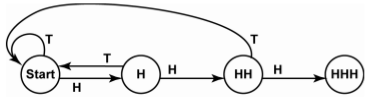
\includegraphics[width=3.5in]{StateDiagramforHHH}
			\end{center}
		
			\caption{Markov chain for HHH as represented by a state diagram \cite{nickerson}}
			\label{perfect_fig}
		\end{figure}

		\begin{figure}[h]
			\begin{center}
				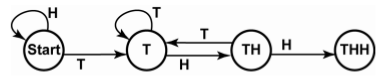
\includegraphics[width=3.5in]{StateDiagramforTHH}
			\end{center}
			
			\caption{Markov chain for THH as represented by a state diagram \cite{nickerson}}
			\label{perfect_fig}
		\end{figure}

		\begin{figure}[h]
			\begin{center}
				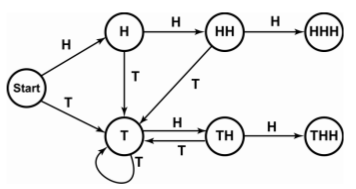
\includegraphics[width=3.5in]{RaceBetweenHHHandTHH}
			\end{center}
			
			\caption{Markov chain for whether HHH or THH appears first \cite{nickerson}}
			\label{perfect_fig}
		\end{figure}

		As we found in our homework, the expected waiting time $E(\tau_S)$ for each sequence of length $n$ can be described as a set of linear equations where $S_0 = 0$. For $1 < k < n-1$,
		$$E(S_k) = \frac{1}{2}E(S_{k-1}) + \frac{1}{2}E(S_{k+1})$$  

		Now consider the probability that player A's sequence comes before player B's sequence. The graph of this game, where the end state is a player finding their sequence, can be represented by figure 3.

		We can use Conway's algorithm to check that the probability that A will precede B in the example sequence is $P(A < B) = .125$. 
 
	\section{Martingale Approach}
		Now we turn to the theory of martingales to study the penney ante problem. Again, let $S$ denote a finite sequence of $n$ coin flips $S = s_1, s_2, ..., s_n$ where each $s_i$ is composed of either $H$ or $T$. We say that the process $S$ is a martingale if the expected waiting time for an element in the sequence of $S$ is finite and if the expected next item in the sequence $s_{k+1}$ conditioned on all previous items is based on the current item $s_k$. 

		\begin{definition}[Martingale \cite{li}]
			A martingale is a sequence of random variables $S = s_1, s_2, ...$ such that for any integer $k$ and for any finite expected value $E(|s_k|)$,
			$$E(s_{k+1} | s_1, ..., s_k) = s_k$$		
		\end{definition}

		Note that although markov chains and martingales are both stochastic processes, they both fundamentally represent different things. A markov chain is a stochastic process such that the expected next step in the process depends only on the current step. A martingale is a stochastic process such that the expected mean value of the next step is equal to the current step. 

	\section{Combinatoric Approach}
		According to Guibas and Odlyzko, the $A \oplus A$ quantity defined in Conway's algorithm represents the period of overlap of A with itself \cite{guibas}. The generalized notion of counting the period of string overlaps is the basis for the combinatorial approach for solving the penney ante problem for a generalized $q$-alphabet. 

		Counting string overlaps also demonstrates the nontransitivity of the game. A remarkable result, if player A chooses string A, player B can choose string B such that $P(B < A)$.
		\begin{theorem}(\cite{guibas})
			If player A chooses string $A = a_1,a_2,...,a_n$, player B can choose a string $B = a_0,a_1,a_2,...,a_{n-1}$ for some $a_0$ for an optimal solution to beat A.
		\end{theorem}

		Furthmore, Guibas and Odlyzko point out that for large $n$, $a_0$ can be chosen so that player B has odds of beating player A of $\frac{q}{q-1}$. This means that no matter which string A chooses, B can choose one that has a greater chance of winning which is why this game is nontransitive. 


	\section{Future Work}
		In this paper we have examined string searching games for 2 and general $q$ alphabet strings of length $n$. However, what happens when searching for a $q$ alphabet string that is biased towards certain letters in the alphabet? This could be an area of further research. Another area of research is examining properties of nontransitive games with the string searching game as an example. I am not quite sure what role I want nontransitivity to play in my paper and I think I will have a better sense of this over time, but for now it looks as if there is enough to consider where an in depth look on nontransitivity would be out of scope for my thesis.

	\begin{thebibliography}{1}
		\bibitem{boyer}
			Boyer, Robert S., and J. Strother Moore. "A Fast String Searching Algorithm." Communications of the ACM 20.10 (1977): 762-72. Web. 
		\bibitem{breen}
			Breen, Stephen, Waterman Michael S., and Zhang Ning. "Renewal Theory for Several Patterns." Journal of Applied Probability 22.1 (1985): 228-34. Web.
		\bibitem{gardner}
			Gardner, Martin. "Mathematical Games: On the Paradoxical Situations That Arise from Nontransitive Relations." Scientific American 10 (1974): 120-25. Print.
		\bibitem{guibas}
			Guibas, L.j, and A.m Odlyzko. "String Overlaps, Pattern Matching, and Nontransitive Games." Journal of Combinatorial Theory, Series A 30.2 (1981): 183-208. Web.  Guibas, L.j, and A.m Odlyzko. "String Overlaps, Pattern Matching, and Nontransitive Games." Journal of Combinatorial Theory, Series A 30.2 (1981): 183-208. Web. 
		\bibitem{li}
			Li, Shuo-Yen Robert. "A Martingale Approach to the Study of Occurrence of Sequence Patterns in Repeated Experiments." The Annals of Probability 8.6 (1980): 1171-176. Web.
		\bibitem{nickerson}
			Nickerson, R. S. "Penney Ante: Counterintuitive Probabilities in Coin Tossing." The UMAP Journal 28.4 (2007): 503-32. JSTOR. Web. 8 Sept. 2016. 
		\bibitem{textbook}
			Levin, David Asher, Y. Peres, and Elizabeth L. Wilmer. Markov Chains and Mixing times. Providence, RI: American Mathematical Society, 2009. Print. 
			
	\end{thebibliography}
\end{document}

 